\documentclass[14pt, a4paper]{article}
\usepackage[russian]{babel}
\usepackage{graphicx}
% \usepackage{tabularx}
\usepackage{layout}
\usepackage[14pt]{extsizes}
\usepackage[hidelinks]{hyperref}
\usepackage{caption}

\usepackage{listings}
\usepackage{xcolor}

\setlength{\emergencystretch}{10pt}
% \usepackage[compact]{titlesec}

\oddsidemargin = 0pt
\marginparwidth = 45pt %57
\textwidth = 467pt
\textheight = 716pt
\topmargin = 0pt %17
\footskip = 30pt %30
\headheight = 0pt %12
\headsep = 0pt %25

\title{Методичка 4}

\definecolor{codegreen}{rgb}{0,0.6,0}
\definecolor{codegray}{rgb}{0.5,0.5,0.5}
\definecolor{codepurple}{rgb}{0.58,0,0.82}
\definecolor{backcolour}{rgb}{0.97,0.97,0.97}

\lstdefinestyle{mystyle}{
    backgroundcolor=\color{backcolour},   
    commentstyle=\color{codegreen},
    keywordstyle=\color{magenta},
    numberstyle=\tiny\color{codegray},
    stringstyle=\color{codepurple},
    basicstyle=\ttfamily\footnotesize,
    breakatwhitespace=false,         
    breaklines=true,                 
    captionpos=b,                    
    keepspaces=true,
    frame=single,                 
    % numbers=left,                    
    % numbersep=5pt,                  
    showspaces=false,                
    showstringspaces=false,
    showtabs=false,                  
    tabsize=2
}

\lstset{style=mystyle}



\begin{document}

\begin{titlepage}
    \topmargin=216pt
    \newpage
    \hangindent=0.7cm
    \huge ИУ-10\\
    Системное\\
    Программное\\
    Обеспечение\\
    \textbf{Системы виртуализации\\ 
    Гипервизоры первого типа\\(продолжение)}

    \vspace{10cm}

    \begin{center}
        \small\textit{Москва, 2022}
    \end{center}
\end{titlepage}
% \layout ##########################################################################################
\section*{На этом уроке}
Рассмотрим примеры гипервизоров первого типа:
\begin{itemize}
    \item Microsoft Hyper-V;
    \item Xen;
    \item KVM.
\end{itemize}
\tableofcontents
\newpage

\section*{Примеры гипервизоров первого типа}
\addcontentsline{toc}{section}{Примеры гипервизоров первого типа}

\subsection*{Microsoft Hyper-V}
\addcontentsline{toc}{subsection}{Microsoft Hyper-V}


\subsubsection*{Микроядерный гипервизор}
\addcontentsline{toc}{subsubsection}{Микроядерный гипервизор}

Ранее мы рассмотрели гипервизор VMware ESXi как весьма удачный и получивший широкое
распространение пример монолитного гипервизора. А теперь обратим внимание на его, в некотором
смысле, антагониста — микроядерный гипервизор Microsoft Hyper-V.

На схеме ниже представлен общий обзор архитектуры среды Hyper-V из \href{https://docs.microsoft.com/ru-ru/virtualization/hyper-v-on-windows/reference/hyper-v-architecture}{официальной документации Microsoft}.

\begin{figure}[h]%current location
    \centering
    \scalebox{1}{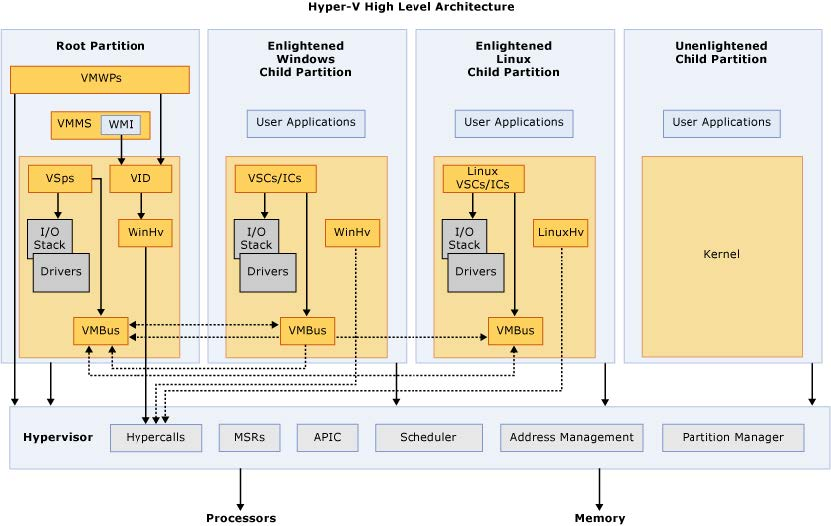
\includegraphics[width=0.8\textwidth]{imgs/1.1.jpg}}
    % \caption*{\textit{Выполнение ПО в разных режимах работы процессора}}
    \label{framework} %framework,fig1
\end{figure}

Как мы видим, сам по себе гипервизор реализует только базовый набор функций, в частности:

\begin{enumerate}
    \item \textbf{Управление разделами} (по сути, гостевыми окружениями или системами), за это отвечает
    Partition manager.
    \item \textbf{Управление памятью} (Address Manager и Memory Service Routine MSR).
    \item \textbf{Диспетчеризация задач} (Scheduler).
    \item \textbf{Управление прерываниями} (Advanced Programmable Interrupt 
    Controller — APIC).
    \item \textbf{Выполнение гипервызовов} (Hypercalls).
\end{enumerate}

Из того, что мы видели в монолитном гипервизоре, тут не хватает как минимум драйверов для
взаимодействия с реальным оборудованием и интерфейса взаимодействия с пользователем или
внешней системой управления гипервизором и гостевыми системами.

Эти функции перенесены из гипервизора в первую гостевую систему, или, как её называют на языке
Hyper-V, корневой раздел. В качестве него выступает одна из операционных систем Microsoft:
Windows 10 на персональном компьютере или Windows Server на сервере. Благодаря этому мы
имеем:

\begin{enumerate}
    \item \textbf{Поддержку широчайшего разнообразия аппаратуры}. По сути, любая аппаратура, на
    которой могут быть запущены названные ОС Microsoft, пригодна для запуска гипервизора
    Microsoft Hyper-V. Для сравнения тут стоит вспомнить весьма ограниченный перечень
    поддерживаемой аппаратуры для запуска VMware ESXi.
    \item \textbf{Развитые и удобные средства управления гипервизором}. Поскольку первая гостевая
    система — полноценная ОС общего назначения (Windows 10 или Windows Server), то не
    удивительно, что интерфейс управления гипервизором может быть выполнен в виде
    обыкновенного приложения для этой ОС. Хороший тому пример — Microsoft Hyper-V Manager.
\end{enumerate}

Интересно отметить, что для обеспечения высокой производительности гостевых систем фактически
необходимо использовать паравиртуализацию. На языке Hyper-V гостевые системы c поддержкой
соответствующей паравиртуализации называются enlightened (в пер. с англ. «просвещённые»). К
таким системам относятся, очевидно, ОС компании Microsoft, а также Linux-дистрибутивы,
использующие ядро версии старше 3.4 и FreeBSD версии старше 10.0 с установленным набором
Linux Integration Services (LIS). Больше деталей можно узнать из \href{https://docs.microsoft.com/ru-ru/windows-server/virtualization/hyper-v/supported-linux-and-freebsd-virtual-machines-for-hyper-v-on-windows}{статьи «Поддерживаемые
виртуальные машины Linux и FreeBSD для Hyper-V в Windows»}.\\


\subsubsection*{Установка гипервизора}
\addcontentsline{toc}{subsubsection}{Установка гипервизора}

Стоит отметить, что гипервизор Hyper-V доступен в двух ипостасях: как отдельный продукт Microsoft
Hyper-V Server и как одна из ролей в Windows Server или Windows 10. Серверная роль — это набор
свойств и сервисов, которые могут использоваться для реализации какой-то конкретной
функциональности сервера. Типичные примеры: веб- или DNS-сервер.

При этом Microsoft Hyper-V Server распространяется бесплатно в виде образа компакт-диска и не
требует покупки лицензии для использования, а роль гипервизора Hyper-V, активируемая в
полноценном Windows Server, требует лицензирования самого Windows Server в соответствии с его
разновидностью. Речь идёт о лицензии на собственно гипервизор. Разумеется, запускаемые гостевые
системы должны быть лицензированы соответствующим образом. То есть гостевые системы с
Linux-дистрибутивами, такие как Ubuntu, CentOS, не требуют покупки дополнительных лицензий, а вот
гостевые системы с Windows требуют приобретения лицензий для каждого экземпляра используемой
ОС внутри виртуальной машины.

На сегодняшний день существуют следующие \href{https://www.microsoft.com/en-us/cloud-platform/windows-server-pricing}{разновидности Windows Server}: Essentials, Standard и
Datacenter. Гипервизор можно \href{https://www.microsoft.com/en-us/evalcenter/evaluate-hyper-v-server-2019}{загрузить с сайта Microsoft}.

По сравнению с ESXi, дистрибутив которого занимает примерно 300 Мбайт, Microsoft Hyper-V Server
выглядит тяжеловесом, так как имеет в 10 раз больший дистрибутив — 3 Гбайт!

\textbf{Microsoft Hyper-V Server} — это, по сути, обыкновенный \href{https://docs.microsoft.com/ru-ru/windows-server/administration/server-core/what-is-server-core}{Windows Server Core}, у которого включена
единственная роль гипервизора Hyper-V, а все остальные компоненты удалены и не могут быть
дополнительно установлены. В том числе отсутствует компонент рабочего стола, так что
единственный доступный интерфейс с пользователем или администратором — это окно стандартной
оболочки cmd.exe. Однако можно подключиться к Microsoft Hyper-V Server по сети и использовать для
дальнейшей настройки и управления виртуальными машинами широкий набор удобных графических
утилит, таких как «Диспетчер Hyper-V» (Hyper-V manager) или System Center Virtual Machine Manager
(SCVMM).

Установка Microsoft Hyper-V Server очень похожа на обычную установку Windows или Windows Server,
с той лишь разницей, что это происходит достаточно быстро за счёт минимального набора
устанавливаемых компонентов. Также не происходит первоначальной настройки рабочего стола
первого пользователя, так как служба рабочего стола отсутствует.

\begin{figure}[h]%current location
    \centering
    \scalebox{0.7}{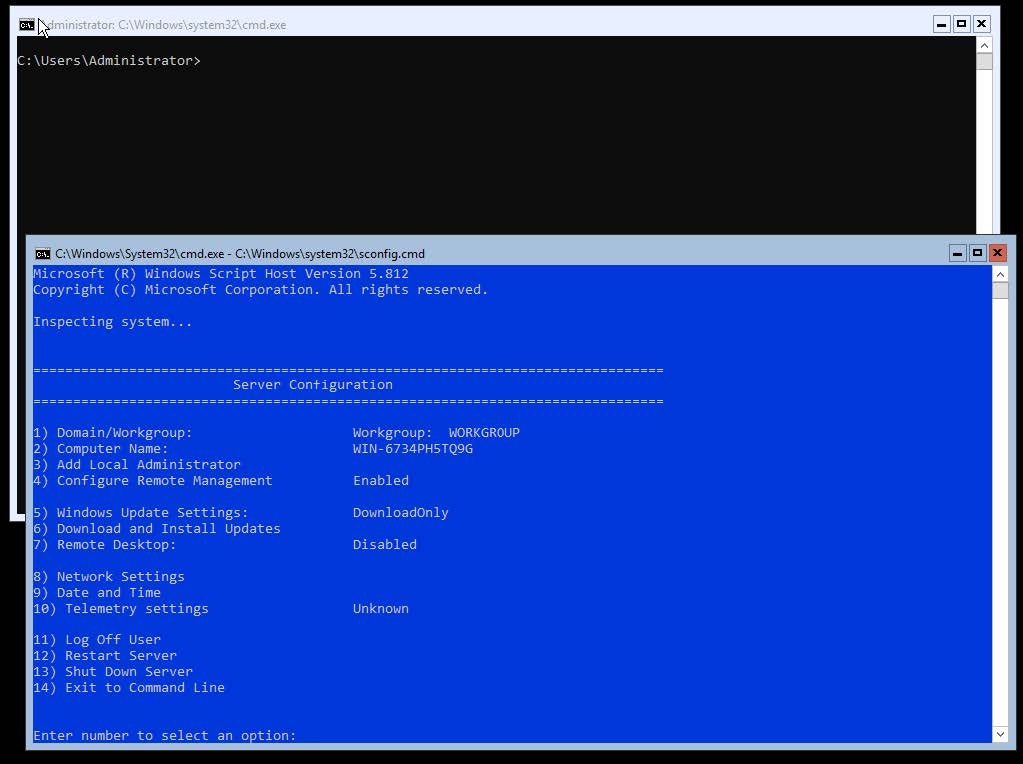
\includegraphics[width=1\textwidth]{imgs/1.2.jpg}}
    % \caption*{\textit{Выполнение ПО в разных режимах работы процессора}}
    \label{1.2} %framework,fig1
\end{figure}

В плане установки полноценный Windows Server мало чем отличается от своего сильно ограниченного
собрата, рассмотренного ранее, разве что после первоначальной установки требуется \href{https://docs.microsoft.com/ru-ru/windows-server/virtualization/hyper-v/get-started/install-the-hyper-v-role-on-windows-server}{активировать
роль Hyper-V гипервизора} и приобрести лицензию на использование самого Windows Server.

Похожим образом можно \href{https://docs.microsoft.com/ru-ru/virtualization/hyper-v-on-windows/quick-start/enable-hyper-v}{активировать роль гипервизора Hyper-V в Windows 10}.\\


\subsubsection*{Использование гипервизора}
\addcontentsline{toc}{subsubsection}{Использование гипервизора}

Для управления гипервизором и гостевыми системами можно использовать разнообразные
инструменты — как разработки Microsoft («Диспетчер Hyper-V» и System Center Virtual Machine
Manager), так и продукты других разработчиков:

\begin{itemize}
    \item \href{http://hv-manager.org/}{HV Manager};
    \item \href{https://www.5nine.com/5nine-manager-standard-edition/}{5Nine Manager};
    \item \href{https://www.manageengine.com/free-hyper-v-configuration/free-hyper-v-configuration-index.html}{Free Hyper-V Server Configuration Tool}.
\end{itemize}

В крайнем случае можно подключиться к серверу Hyper-V RDP-клиентом и установить все настройки,
как если бы к данному серверу был локальный доступ.

\begin{figure}[h]%current location
    \centering
    \scalebox{0.7}{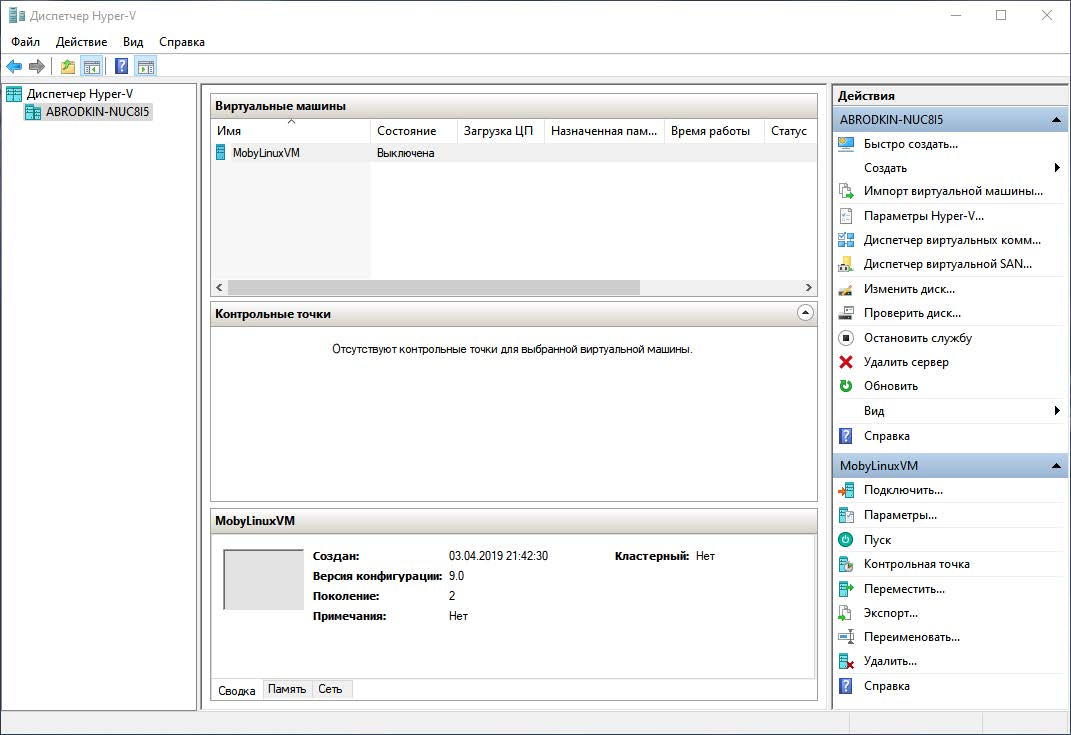
\includegraphics[width=1\textwidth]{imgs/1.3.jpg}}\\
    % \caption*{\textit{Выполнение ПО в разных режимах работы процессора}}
    \label{1.3} %framework,fig1
\end{figure}

\subsubsection*{Создание виртуальных машин}
\addcontentsline{toc}{subsubsection}{Создание виртуальных машин}

Рекомендуем ознакомиться с \href{https://docs.microsoft.com/en-us/windows-server/virtualization/hyper-v/get-started/create-a-virtual-machine-in-hyper-v}{официальной документацией Microsoft}, где подробно разбираются
возможные варианты создания виртуальных машин.

Для удобства пользователей настольных версий Windows, начиная с версии Windows 10 Fall Creators
Update (Windows 10 версии 1709), доступна установка в одно нажатие некоторых популярных
Linux-дистрибутивов. На момент написания данного материала это были Ubuntu 18.04 LTS и Ubuntu
19.04. Имеется в виду desktop version в противовес серверному варианту (Windows server).

\begin{figure}[h]%current location
    \centering
    \scalebox{1}{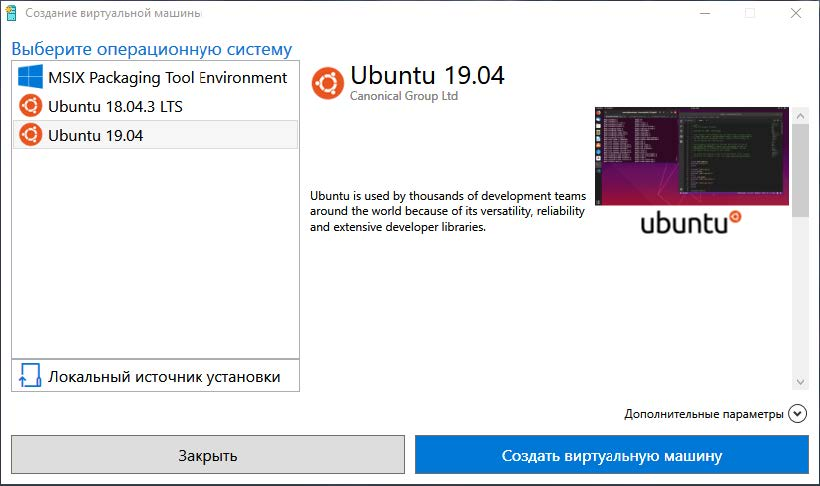
\includegraphics[width=0.49\textwidth]{imgs/1.4.jpg}}
    \scalebox{1}{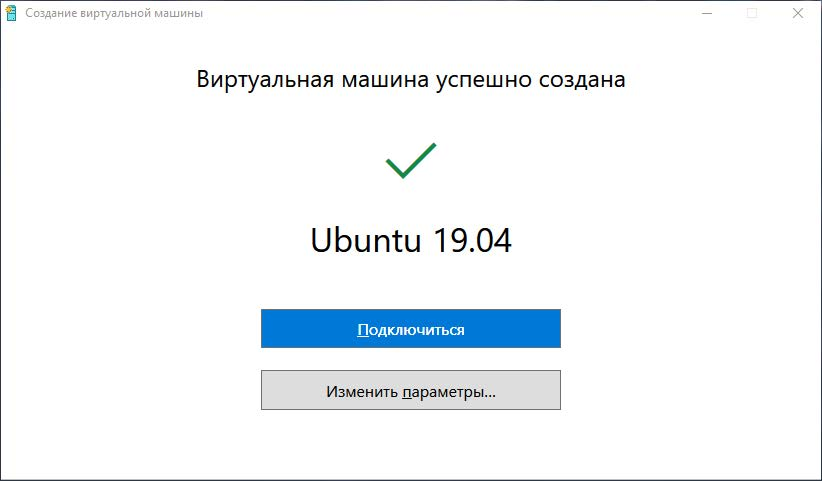
\includegraphics[width=0.49\textwidth]{imgs/1.5.jpg}}
    % \caption*{\textit{Выполнение ПО в разных режимах работы процессора}}
    \label{1.4 1.5} %framework,fig1
\end{figure}

Или же можно запустить «Диспетчер Hyper-V» и вручную настроить все параметры. Этот метод будет
отлично работать в Windows 10 и полноценном Windows Server, в то время как в Windows Hyper-V
Server невозможен непосредственный запуск «Диспетчера Hyper-V» в силу отсутствия графического
рабочего стола. Тем не менее «Диспетчер Hyper-V» можно запустить на любой другой машине под
управлением 64-битных Windows 10 версий Pro или Enterprise и управлять Windows Hyper-V Server
удалённо, как если бы программа управления была запущена локально прямо на сервере.

\begin{figure}[h]%current location
    \scalebox{1}{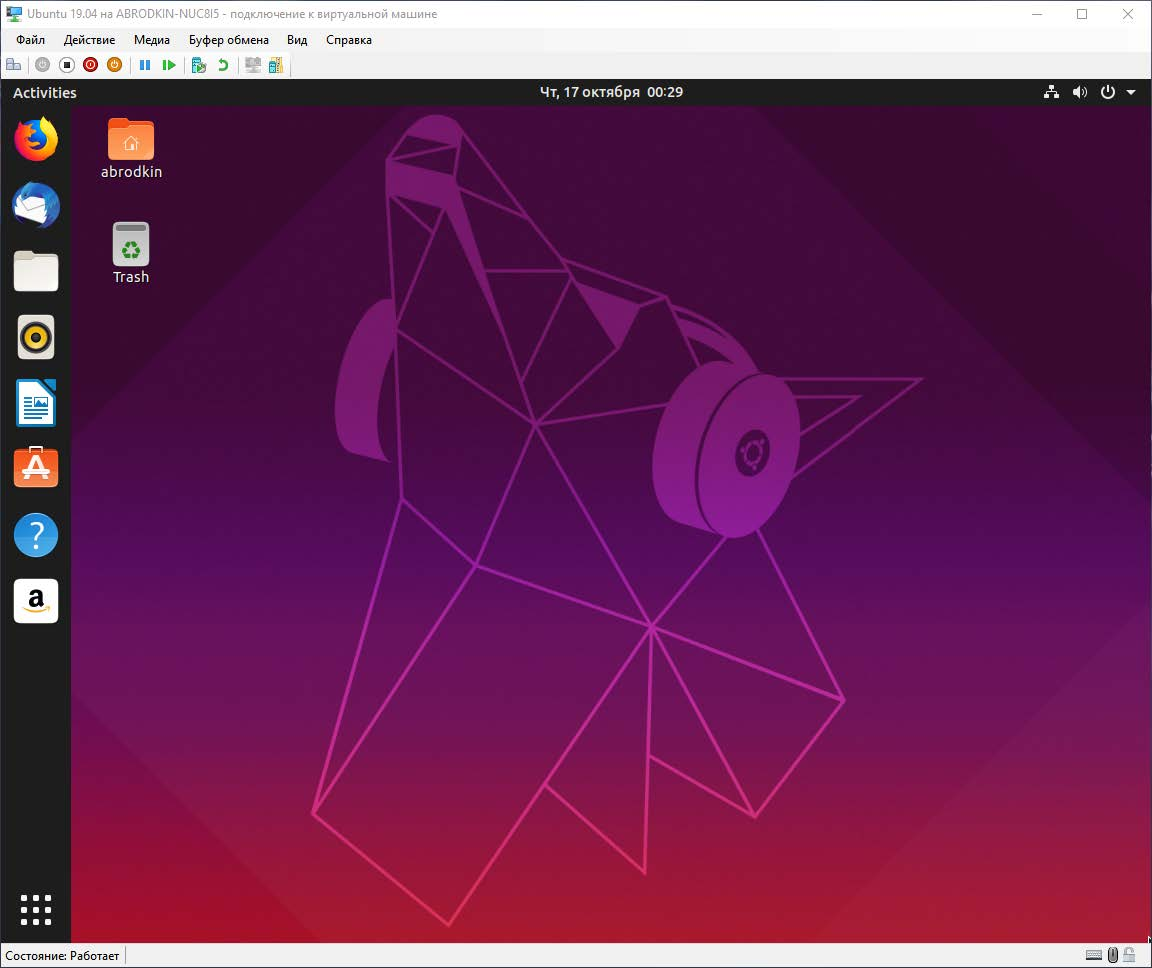
\includegraphics[width=0.5\textwidth]{imgs/1.6.jpg}}    % \caption*{\textit{Выполнение ПО в разных режимах работы процессора}}
    \label{1.6} %framework,fig1
\end{figure}

Однако в условиях реальных дата-центров или серверных окружений, о которых мы в основном
говорим в данном курсе, чаще используются скрипты на Windows PowerShell как гораздо более
эффективный метод. Как мы уже отмечали ранее, использование скриптов позволяет избежать
хождения по меню графического клиента, использовать заранее заготовленные шаблоны или даже
параметризовать некоторые параметры и производить необходимые действия автоматически.
Ознакомьтесь с \href{https://docs.microsoft.com/en-us/powershell/module/hyper-v/new-vm}{примерами использования команды New-VM}.

Аналогично можно создавать копии имеющихся виртуальных машин, импортировать или
экспортировать виртуальные машины Hyper-V. При желании импортировать виртуальные машины в
формате OVF придётся их сначала конвертировать в формат Hyper-V, что может оказаться не самой
простой процедурой. Дело в том, что ранее существовавший для решения данной задачи инструмент
\href{https://docs.microsoft.com/en-us/previous-versions/windows/it-pro/windows-server-2012-r2-and-2012/dn874008(v%3Dws.11)}{Microsoft Virtual Machine Converter} (MVMC) был объявлен устаревшим и его поддержка прекратилась
ещё в 2017 году. Компания Microsoft официально рекомендует использовать сервис \href{https://azure.microsoft.com/en-us/services/site-recovery/}{Azure Site
Recovery}. Как вариант, можно воспользоваться одним из нескольких решений от других
разработчиков, например, \href{https://www.5nine.com/5nine-cloud-migration-free/}{5nine Cloud Migration Free} или \href{https://www.starwindsoftware.com/starwind-v2v-converter}{StarWind V2V Converter}.\\

\subsubsection*{Резюме}
\addcontentsline{toc}{subsubsection}{Резюме}

Microsoft Hyper-V — современный высокопроизводительный гипервизор, который находит всё более
широкое применение в системах серверной виртуализации. Его неоспоримые достоинства: высокая
интегрированность с другими решениями компании Microsoft и высокая эффективность, не
уступающая другим гипервизорам. Как показывает практика, системы серверной виртуализации на
основе Hyper-V становятся всё более популярными. Кроме того, компания Microsoft не просто
занимается разработкой Hyper-V для использования их клиентами, но построила и развивает
облачную платформу Microsoft Azure, основой которой служит как раз гипервизор Microsoft Hyper-V.
Это даёт надежду, что качество и эффективность гипервизора будут со временем только улучшаться.\newpage

\subsection*{Xen}
\addcontentsline{toc}{subsection}{Xen}

\begin{figure}[h]%current location
    \centering
    \scalebox{1}{
\includegraphics[width=0.3\textwidth]{imgs/2.0.jpg}}
    \caption*{\textit{Логотип Xen}}
    \label{2.0} %framework,fig1
\end{figure}

\href{https://ru.wikipedia.org/wiki/Xen}{Xen} (произносится «зэн») — это кроссплатформенный гипервизор, разработанный в компьютерной
лаборатории Кембриджского университета и распространяемый на условиях лицензии GPL.


\subsubsection*{Микроядерный гипервизор}
\addcontentsline{toc}{subsubsection}{Микроядерный гипервизор}


По своей архитектуре Xen похож на Microsoft Hyper-V, хотя было бы правильнее говорить о том, что
Microsoft Hyper-V чем-то очень напоминает Xen, потому что Hyper-V был явлен публике только в 2008
году, когда Xen уже имел версию 3.2.

\begin{figure}[h]%current location
    \centering
    \scalebox{1}{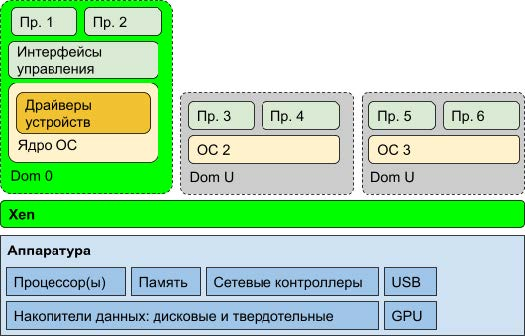
\includegraphics[width=0.8\textwidth]{imgs/2.1.jpg}}
    \label{2.1} %framework,fig1
\end{figure}

Сам по себе гипервизор очень компактен: всего ~65 000 строк кода для процессоров ARM и ~300 000
строк кода для процессоров с архитектурой x86. Соответственно, он обладает минимальной
функциональностью: управлением памятью, состоянием процессора, таймерами и прерываниями.
Значительную часть возможностей системы реализует первая привилегированная гостевая система,
называемая Dom0 (от англ. Domain 0 — «нулевой домен»). В том числе в Dom0 системой
осуществляется управление гипервизором. Все остальные системы в DomU (от англ. Unprivileged
domain — «непривилегированный домен») не имеют каких-либо особенных привилегий и
используются для запуска обыкновенных гостевых систем.


Существенное отличие Xen от Microsoft Hyper-V заключается в поддержке нескольких процессорных
архитектур. Microsoft Hyper-V может работать только на 64-битной x86 платформе, то есть фактически
только на процессорах производства Intel и AMD. А Xen может быть запущен на 32-битной или
64-битной платформе ARM или x86. При этом управляющей системой в Dom0, как правило, бывает
основанный на ядре Linux дистрибутив, хотя возможно использование в этой роли и других ОС, таких
как NetBSD и OpenSolaris.


Важной особенностью Xen с самого начала была возможность использовать паравиртуализованные
устройства (PV Guests), что давало существенный выигрыш в производительности по сравнению с
другими гипервизорами, эмулировавшими устройства ввода-вывода. Разумеется, это требовало
поддержки паравиртуализованных Xen-устройств в гостевых системах. Как мы знаем, в настоящее
время все современные гипервизоры предоставляют возможность использовать
паравиртуализованные устройства для достижения высокой производительности, так что данная
особенность Xen не уникальна.


\subsubsection*{Установка гипервизора}
\addcontentsline{toc}{subsubsection}{Установка гипервизора}


Так как Xen, как и рассмотренный ранее Microsoft Hyper-V,— микроядерный гипервизор, то есть, по
сути, промежуточный слой между аппаратурой и гостевыми окружениями, невозможно представить
его без полноценной операционной системы, запущенной в привилегированном окружении Dom0. А
потому, как и в случае Hyper-V, установка Xen выглядит во многом как установка обычного
Linux-дистрибутива. В нём либо с самого начала, либо после дополнительной настройки используется
специальным образом модифицированное ядро. Загрузчик стартует не ядро Linux, а гипервизор,
который после первоначальной инициализации оборудования загружает и запускает ядро Linux в
первом привилегированном окружении Dom0.


Есть два варианта установки гипервизора Xen:

\begin{enumerate}
    \item \textbf{При помощи специально подготовленного дистрибутива}. Типичный пример — \href{https://www.citrix.com/products/citrix-hypervisor/}{Citrix
    Hypervisor} или его вариант, подготовленный сообществом, — \href{https://xcp-ng.org/}{XCP-ng} (Xen Cloud Platform, new
    generation). По сути, и тот, и другой вариант — дистрибутивы CentOS с предварительно
    настроенным установщиком, ядром ОС Linux, готовым для работы поверх гипервизора Xen, и
    необходимым дополнительным ПО.
\end{enumerate}


Для установки потребуется как минимум 100 Гбайт места на диске для локального хранилища данных
всех доменов, иначе при объёме диска менее 50 Гбайт установщик выдаст сообщение о недостатке
свободного места и прервёт процесс установки. А при диске объёмом 50 Гбайт после завершения
установки останется всего порядка 8 Гбайт для гостевых систем, чего недостаточно даже для Xen
Orchestra Appliance — гостя с веб-интерфейсом управления гипервизором Xen. Причём для установки
внутри KVM необходимо выбрать тип диска SCSI вместо варианта по умолчанию Virtio. Драйвер Virtio
отсутствует в исходном дистрибутиве, и такое устройство не будет распознано установщиком.


Xen можно установить и запустить внутри другого гипервизора, используя так называемую вложенную
виртуализацию, о ней мы поговорим позже. \href{https://github.com/xcp-ng/xcp/wiki/Testing-XCP-ng-in-Virtual-Machine-(Nested-Virtualization)#nested-xcp-ng-using-qemukvm}{Советы для запуска Xen на разных гипервизорах}.


\begin{enumerate}
    \item[2.] \textbf{При помощи дополнительной настройки обыкновенного Linux-дистрибутива}:
    \href{https://wiki.debian.org/Xen}{Debian}/\href{https://help.ubuntu.com/community/Xen}{Ubuntu}, RHEL/\href{https://wiki.centos.org/HowTos/Xen/Xen4QuickStart}{CentOS}/\href{https://wiki.xen.org/wiki/Fedora_Host_Installation}{Fedora}, OpenSUSE и так далее. В этом случае сначала
    устанавливается Linux-дистрибутив на выбор, а затем гипервизор и модифицированное ядро
    Linux. Инструкции для разных дистрибутивов могут значительно меняться. Кроме того, со
    временем могут меняться команды, названия устанавливаемых пакетов, местоположение
    конфигурационных файлов и т. д. Так что стоит искать инструкции для конкретной версии
    выбранного дистрибутива, чтобы избежать дополнительных временных затрат на выяснение
    причин неудач и переустановку с нуля. 
\end{enumerate}


Статья об установке Xen на Ubuntu последний раз обновлялась в 2015 году, так что может быть
устаревшей. Стоит обратить внимание на документацию для Debian, поскольку Ubuntu использует
Debian как основу. Статья об установке Xen на Fedora последний раз обновлялась в ноябре 2014 года.
Скорее всего, она мало пригодна при использовании со свежими версиями Fedora.


При старте сервера с установленным гипервизором Xen можно наблюдать следующий вывод в
консоль отладки (по умолчанию это монитор):

\begin{lstlisting}
(XEN) Xen version 4.12.1_02-lp151.2.3 (abuild@suse.de) (gcc (SUSE Linux) 7.4.1 20190424 [gcc-7-branch revision 270538]) debug=n Wed Oct 2 08:37:47 UTC 2019
(XEN) Latest ChangeSet:
(XEN) Bootloader: GRUB2 2.02
(XEN) Command line: vga=gfx-1024x768x16
(XEN) Xen image load base address: 0
(XEN) Video information:
(XEN) VGA is graphics mode 1024x768, 16 bpp
(XEN) Disc information:
(XEN) Found 1 MBR signatures
(XEN) Found 1 EDD information structures
(XEN) Xen-e820 RAM map:
(XEN) 0000000000000000 - 000000000009fc00 (usable)
(XEN) 000000000009fc00 - 00000000000a0000 (reserved)
(XEN) 00000000000f0000 - 0000000000100000 (reserved)
(XEN) 0000000000100000 - 00000000bffd9000 (usable)
(XEN) 00000000bffd9000 - 00000000c0000000 (reserved)
(XEN) 00000000feffc000 - 00000000ff000000 (reserved)
(XEN) 00000000fffc0000 - 0000000100000000 (reserved)
(XEN) 0000000100000000 - 0000000240400000 (usable)
(XEN) New Xen image base address: 0xbf800000
(XEN) ACPI: RSDP 000F69C0, 0014 (r0 BOCHS )
(XEN) ACPI: RSDT BFFE13E7, 002C (r1 BOCHS BXPCRSDT 1 BXPC 1)
(XEN) ACPI: FACP BFFE1263, 0074 (r1 BOCHS BXPCFACP 1 BXPC 1)
(XEN) ACPI: DSDT BFFDFDC0, 14A3 (r1 BOCHS BXPCDSDT 1 BXPC 1)
(XEN) ACPI: FACS BFFDFD80, 0040
(XEN) ACPI: APIC BFFE1357, 0090 (r1 BOCHS BXPCAPIC 1 BXPC 1)
(XEN) System RAM: 8195MB (8392160kB)
(XEN) Domain heap initialised
...
(XEN) Dom0 has maximum 4 VCPUs
(XEN) Initial low memory virq threshold set at 0x4000 pages.
(XEN) Scrubbing Free RAM in background
(XEN) Std. Loglevel: Errors and warnings
(XEN) Guest Loglevel: Nothing (Rate-limited: Errors and warnings)
(XEN) Xen is relinquishing VGA console.
(XEN) *** Serial input to DOM0 (type 'CTRL-a' three times to switch input)
(XEN) Freed 496kB init memory
\end{lstlisting}

А после окончания загрузки гипервизора стартует ядро ОС Linux в Dom0:

\begin{lstlisting}
[ 0.000000] Linux version 4.12.14-lp151.28.20-default (geeko@buildhost) (gcc version 7.4.1 20190424 [gcc-7-branch revision 270538] (SUSE Linux) ) #1 SMP Tue Oct 8 05:42:34 UTC 2019 (2982b5d)
[ 0.000000] Command line: root=UUID=57a0f387-74f3-46fb-9731-fedbeceb2fb9 splash=silent resume=/dev/disk/by-path/pci-0000:00:07.0-part3 quiet mitigations=auto
[ 0.000000] x86/fpu: Supporting XSAVE feature 0x001: 'x87 floating point registers'
[ 0.000000] x86/fpu: Supporting XSAVE feature 0x002: 'SSE registers'
[ 0.000000] x86/fpu: Supporting XSAVE feature 0x004: 'AVX registers'
[ 0.000000] x86/fpu: xstate_offset[2]: 576, xstate_sizes[2]: 256
[ 0.000000] x86/fpu: Enabled xstate features 0x7, context size is 832 bytes, using 'standard' format.
[ 0.000000] Released 0 page(s)
[ 0.000000] e820: BIOS-provided physical RAM map:
[ 0.000000] Xen: [mem 0x0000000000000000-0x000000000009efff] usable
[ 0.000000] Xen: [mem 0x000000000009fc00-0x00000000000fffff] reserved
[ 0.000000] Xen: [mem 0x0000000000100000-0x00000000bffd8fff] usable
[ 0.000000] Xen: [mem 0x00000000bffd9000-0x00000000bfffffff] reserved
[ 0.000000] Xen: [mem 0x00000000fec00000-0x00000000fec00fff] reserved
[ 0.000000] Xen: [mem 0x00000000fee00000-0x00000000feefffff] reserved
[ 0.000000] Xen: [mem 0x00000000feffc000-0x00000000feffffff] reserved
[ 0.000000] Xen: [mem 0x00000000fffc0000-0x00000000ffffffff] reserved
[ 0.000000] Xen: [mem 0x0000000100000000-0x00000002403fffff] usable
[ 0.000000] NX (Execute Disable) protection: active
[ 0.000000] SMBIOS 2.8 present.
[ 0.000000] DMI: QEMU Standard PC (i440FX + PIIX, 1996), BIOS 1.10.2-1ubuntu1 04/01/2014
[ 0.000000] Hypervisor detected: Xen PV
[ 0.000000] tsc: Fast TSC calibration using PIT
[ 0.000000] e820: update [mem 0x00000000-0x00000fff] usable ==> reserved
[ 0.000000] e820: remove [mem 0x000a0000-0x000fffff] usable
[ 0.000000] e820: last_pfn = 0x240400 max_arch_pfn = 0x400000000
\end{lstlisting}

Стоит отметить, что сам по себе гипервизор Xen, будучи реализацией микроядерной архитектуры, —
то есть он реализует минимальный набор функциональности — недостаточен для полноценной
реализации системы виртуализации. Для неё требуется ещё и соответствующим образом
модифицированная система в Dom0 с набором необходимого инструментария. Другими словами,
возможная в теории установка Xen вместе со случайным Linux-дистрибутивом может оказаться не
самым лучшим решением с точки зрения и простоты установки, и удобства дальнейшего
использования. Использование проприетарного Citrix Hypervisor или разрабатываемого сообществом
XCP-ng рекомендуется для любого типа использования: и для ознакомления, и для реальных
«боевых» систем.\\

\subsubsection*{Использование гипервизора}
\addcontentsline{toc}{subsubsection}{Использование гипервизора}


Как мы знаем, использование гипервизора сводится к запуску поверх него гостевых систем.
Соответственно, основные действия, производимые с гипервизором, — это управление гостевыми
системами: их создание, уничтожение, перенос, клонирование и т. д.

В случае гипервизора Xen существует несколько широко используемых методов управления:
\begin{enumerate}
    \item \textbf{Xsconsole} — текстовая консоль при непосредственном доступе к серверу, когда картинка
    выводится на подключённый монитор, а ввод производится с клавиатуры, или удалённое
    подключение по SSH. После подключения по SSH нужно выполнить команду xsconsole. Хотя
    интерфейс Xsconsole выглядит весьма аскетично, он предоставляет минимальный набор
    инструментов для решения простых задач, таких как запуск, остановка, перезагрузка и
    миграция виртуальных машин, просмотр данных о хосте, изменение сетевых настроек и т. д.
    Также можно переключиться в режим командной строки хоста и выполнять любые команды.
    Чем-то Xsconsole напоминает DCUI (Direct Console User Interface) из VMware ESXi, при этом он
    предоставляет больше возможностей в стандартном интерфейсе и даёт неограниченные
    возможности при переключении в командную консоль хоста (на самом деле Dom0).
    \begin{figure}[h]%current location
        \centering
        \scalebox{1}{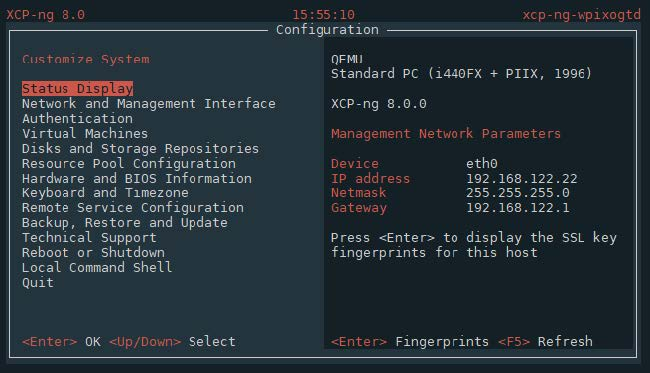
\includegraphics[width=0.8\textwidth]{imgs/2.2.jpg}}
        \label{2.2} %framework,fig1
    \end{figure}
    \item \textbf{Xen tools} — это набор утилит, предназначенных для полноценного управления гипервизором
    Xen и его гостевыми системами. При установке Citrix XenServer или XCP-ng эти утилиты
    изначально доступны в Dom0, а при установке Xen поверх стандартного Linux-дистрибутива
    необходимо дополнительно установить их. Обычно это делается при помощи пакетного
    менеджера используемого дистрибутива. Например, в Debian нужно выполнить команду
    \colorbox{backcolour}{apt-get install xen-tools}.
    \item \textbf{XenCenter/XenAdmin} — графический клиент для ОС Windows. Позволяет подключаться к
    нескольким удалённым серверам Xen, управлять ими и гостевыми системами на них.
    XenCenter возможно использовать только с Citrix Xen Hypervisor, в то время как XenAdmin (по
    сути, форк XenCenter от разработчиков XCP-ng) отлично работает и с Citrix Hypervisor, и с
    XCP-ng.
    \begin{figure}[h]%current location
        \centering
        \scalebox{1}{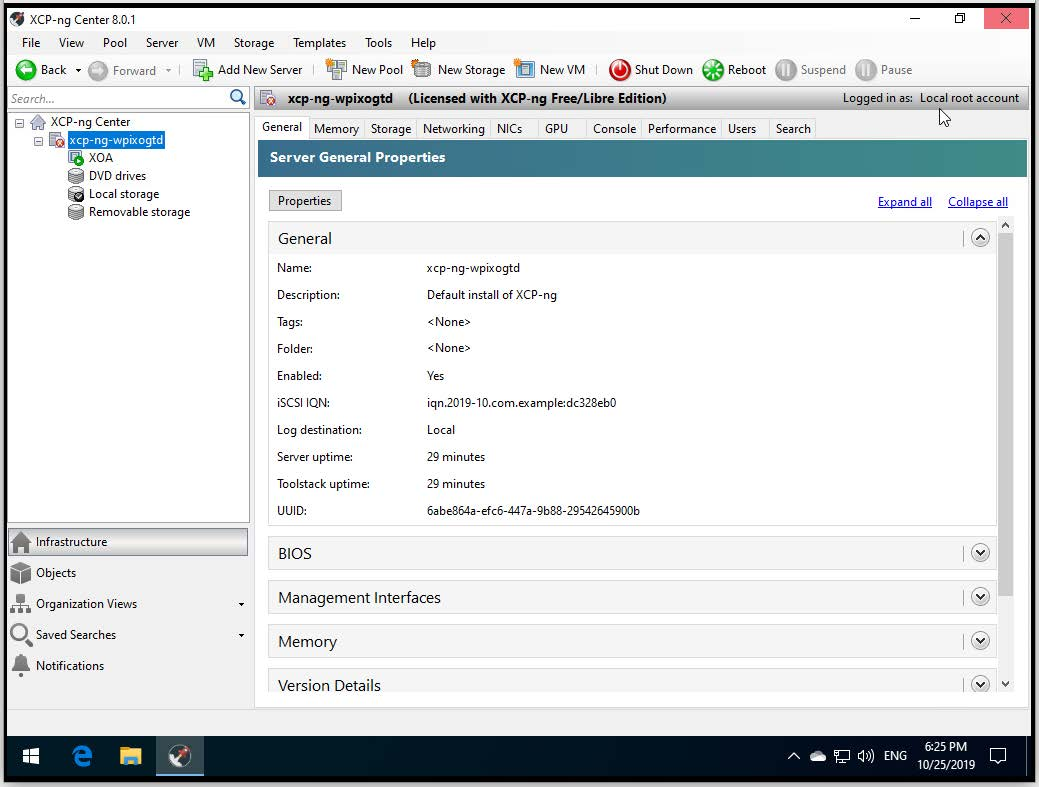
\includegraphics[width=0.8\textwidth]{imgs/2.3.jpg}}
        \label{2.3} %framework,fig1
    \end{figure}
    \item \textbf{Xen Orchestra} — веб-интерфейс для гипервизора Xen. Он устанавливается в виде appliance,
    то есть заранее настроенного образа виртуальной машины, готового к использованию. Таким
    образом, установив Xen Orchestra, мы уже получим первую гостевую систему. Более того,
    поскольку Xen Orchestra запущена в отдельной виртуальной машине, IP-адрес
    веб-интерфейса отличается от адреса непосредственно хозяйского сервера с гипервизором
    Xen.
    \begin{figure}[h]%current location
        \centering
        \scalebox{1}{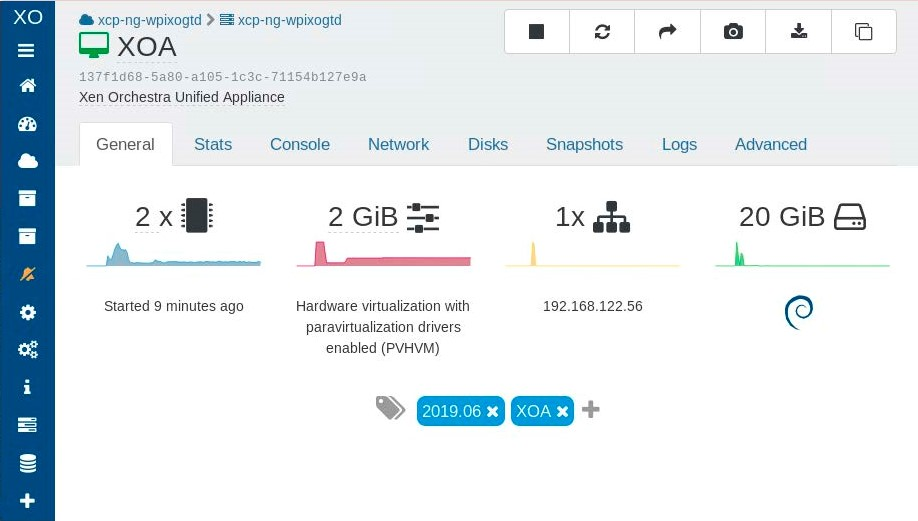
\includegraphics[width=0.8\textwidth]{imgs/2.4.jpg}}
        \label{2.4} %framework,fig1
    \end{figure}
    \item \href{https://libvirt.org/}{libvirt} — универсальная библиотека для работы с самыми разнообразными системами
виртуализации. В теории имеет поддержку Xen, но могут быть нюансы. Например, нам не
удалось её использовать с XCP-ng 8.0 так как не оказалось необходимого драйвера для libvirt.
Впрочем, при установке Xen поверх стандартных дистрибутивов, возможно, что-то и получится
— всё зависит от того, как сконфигурирована библиотека libvirt перед сборкой.\\
\end{enumerate}

\subsubsection*{Создание виртуальных машин}
\addcontentsline{toc}{subsubsection}{Создание виртуальных машин}

Гостевые виртуальные машины можно создавать либо из любого имеющегося графического
интерфейса пользователя, конфигурируя их шаг за шагом, либо при помощи так называемого \href{https://wiki.xenproject.org/wiki/XAPI_Command_Line_Interface}{XAPI} и
специальной утилиты XE. Как и в случае ранее рассмотренных виртуальных машин, возможно
создавать гостевые системы из заранее подготовленных шаблонов, можно \href{https://docs.citrix.com/en-us/xencenter/7-1/vms-about.html}{клонировать имеющиеся
виртуальные машины}, а также импортировать и \href{https://docs.citrix.com/en-us/xencenter/7-1/vms-exportimport.html}{экспортировать виртуальные машины}, используя
стандартные форматы XVA (Citrix Xen appliance format) или OVF/OVA.

\subsubsection*{Резюме}
\addcontentsline{toc}{subsubsection}{Резюме}

Гипервизор Xen — это мощное и гибкое решение для серверной виртуализации, проверенное
временем и множеством реальных пользователей, в том числе и таких, как компания Amazon. В
отличие от гипервизора компании Microsoft, Xen, будучи ПО с открытым исходным кодом, удобен для
глубокого изучения своего внутреннего устройства. Он получает новые возможности, улучшения
имеющейся функциональности и исправления обнаруженных проблем усилиями сообщества. Именно
поэтому Xen может работать с большим набором форматов и имеет хорошо документированные и
развитые инструменты управления.

Ещё недавно позиции Xen казались нерушимыми. Пусть он и не претендовал на долю VMware, но был
весьма привлекателен на фоне не очень большой группы весьма молодых конкурентов, таких как
Microsoft Hyper-V и KVM, за счёт высокой производительности. Она обеспечивалась поначалу
использованием паравиртуализации — PV Guests (Paravirtualization), затем аппаратной поддержкой
виртуализации — HVM Guests (Hardware-assisted virtualization), и наконец, совместив лучшее из двух
миров, — PVH Guests (Paravirtualized Hardware-assisted virtualization). Одним из крупнейших
пользователей XEN была компания Amazon, которая до 2018 года применяла Xen в качестве
основного гипервизора своего облачного сервиса Amazon Elastic Compute Cloud (Amazon EC2). Но со
временем конкурирующие решения стали более зрелыми, то есть более функциональными и
быстрыми, при этом сохранив свои изначальные преимущества: лёгкость установки и использования.

Что интересно, в конце 2017 года компания Amazon объявила о введении в строй нового поколения
элементов инфраструктуры облачного сервиса \href{http://aws_writes_new_kvm_based_hypervisor_to_make_its_cloud_go_faster/}{Amazon Elastic Compute Cloud (Amazon EC2)}, которое
базируется на использовании гипервизора KVM (Kernel-based Virtual Machine) вместо ранее
применяемого Xen. Со временем новый гипервизор планируется задействовать и для других типов
окружений Amazon EC2.\newpage

\subsection*{KVM}
\addcontentsline{toc}{subsection}{KVM}

\begin{figure}[h]%current location
    \centering
    \scalebox{1}{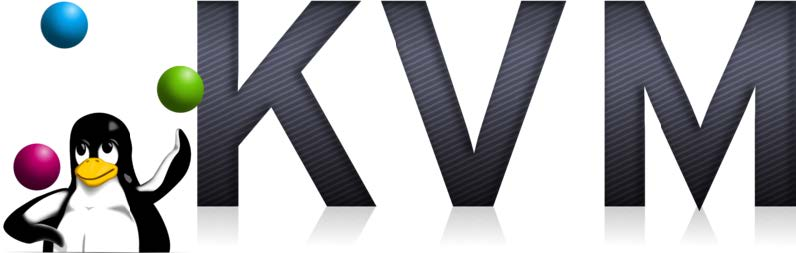
\includegraphics[width=0.5\textwidth]{imgs/3.0.jpg}}
    \caption*{\textit{Логотип KVM}}
    \label{3.0} %framework,fig1
\end{figure}

KVM (Kernel Virtual Machine) — это модуль ядра ОС Linux, который позволяет ядру ОС выполнять роль
гипервизора. Он был анонсирован Ави Кивити 19 октября 2006 года в \href{http://lkml.iu.edu/hypermail/linux/kernel/0610.2/1369.html}{рассылке разработчиков ядра
ОС Linux} и стал неотъемлемой частью исходных текстов ядра Linux, начиная с версии 2.6.20,
выпущенной 5 февраля 2007 года. В отличие от гипервизоров VMware и Xen, KVM со своей первой
версии полагался на реализацию аппаратного ускорения виртуализации в центральном процессоре,
то есть KVM никогда не поддерживал бинарную трансляцию или полную паравиртуализацию гостевой
системы.

В своей первой реализации KVM поддерживал только процессоры компании Intel с расширением
VT-x, однако вскоре была добавлена поддержка процессоров производства AMD с набором
расширений SVM, а позже KVM был портирован на многие другие процессорные архитектуры, такие
как ARM (32- и 64-битные версии), PowerPC, IA-64 (Intel Itanium), IBM System/390. В настоящее время
продолжается активная работа по развитию KVM на уже поддерживаемых архитектурах, а также
добавляется поддержка новых архитектур, в частности, \href{https://lwn.net/Articles/797797/}{RISC-V}.

Интересно отметить, что разработка KVM началась в момент, когда гипервизор Xen был де-факто
единственным решением для виртуализации с открытым исходным кодом. Однако ввиду отсутствия в
то время процессоров с аппаратной поддержкой виртуализации его внутреннее устройство обладало
целым набором особенностей или даже недостатков. В частности, это необходимость использовать в
управляющей системе Dom0 значительно модифицированное ядро ОС, посредством которого
происходила работа с устройствами ввода-вывода и т. д. Ввиду скорого появления процессоров с
поддержкой аппаратного ускорения виртуализации Ави Кивити решил создать свой гипервизор с
чистого листа, с одной стороны, используя новую функциональность аппаратуры процессоров, а с
другой стороны, максимально используя имеющиеся механизмы обыкновенного ядра Linux.

Действительно, ядро ОС уже имеет весьма совершенные подсистемы управления памятью,
планирования выполнения процессов, управления энергопотреблением системы и т. д. По сути,
модуль KVM — это драйвер, позволяющий приложению пользователя использовать расширения
процессора для аппаратного управления виртуализацией. Однако этого недостаточно для реализации
полноценной системы виртуализации, которая по определению моделирует полноценную
вычислительную систему, а не только центральный процессор. В случае KVM эмуляция системы в
целом выполняется при помощи QEMU, который служит полноценным эмулятором самой
разнообразной аппаратуры, в том числе процессоров многих архитектур, а также реальных и
абстрактных устройств ввода-вывода.

Разработчики гипервизора KVM не только использовали имеющуюся функциональность ядра Linux,
но и добавляли улучшения, впоследствии ставшие важными особенностями самого ядра. Хороший
тому пример — THP (Transparent HugePage). Это использование страниц MMU большего размера для
снижения издержек на обработку «отказов страницы» (page fault).\\

\subsubsection*{QEMU}
\addcontentsline{toc}{subsubsection}{QEMU}

На QEMU хочется остановиться немного подробнее. Сам по себе QEMU — это полноценный
гипервизор второго типа, то есть работающий поверх хозяйской операционной системы. Он
выполняет быструю бинарную трансляцию бинарного кода гостевой системы. Отсюда и название
QEMU — это сокращение от Quick EMUlator, «быстрый эмулятор». Относительно высокая скорость
исполнения кода гостевой системы достигается за счёт однократной бинарной трансляции с
последующим использованием сохранённых (закешированных) фрагментов транслированного кода.
Тем не менее эмуляция по определению значительно проигрывает в производительности исполнению
кода непосредственно реальным процессором и, в зависимости от используемых тестов, QEMU в
режиме эмуляции оказывается в разы, десятки раз или даже на несколько порядков медленнее.

Но эмуляция процессора — это только небольшая часть возможностей QEMU. Вторая важная
составляющая QEMU как полноценного эмулятора полной вычислительной системы — это эмуляция
аппаратуры. Первое, что приходит в голову, — это симуляция некоего стандартного набора устройств,
таких как клавиатура, манипулятор типа «мышь», монитор (экран), накопитель данных (HDD или
SSD), сетевые контроллеры и так далее. Это позволит использовать стандартное
немодифицированное ПО в гостевой системе. И действительно, QEMU может эмулировать
достаточно широкий спектр реального оборудования, с перечнем которого можно ознакомиться в
\href{https://en.wikibooks.org/wiki/QEMU/Devices}{официальной документации}.

\subsubsection*{VirtIO}
\addcontentsline{toc}{subsubsection}{VirtIO}

Отдельная категория оборудования — это устройства типа \href{https://en.wikibooks.org/wiki/QEMU/Devices/Virtio}{VirtIO}. Даже в исходном коде и
официальной документации встречается различное написание: Virtio, VirtIO или virtio. По сути, VirtIO
— это платформа для реализации паравиртуализированных устройств. В её основе универсальный
механизм обмена данными между гостевой и хозяйскими системами, поверх которого реализованы
конкретные классы устройств: сетевые контроллеры, устройства хранения данных, генераторы
случайных чисел и так далее.

Причём, поскольку речь идёт о паравиртуализации, в гостевой системе необходимо иметь
дополнительные драйверы VirtIO-устройств, так как VirtIO-устройства обычно не имеют своей
реализации в реальной аппаратуре. С другой стороны, производительность таких виртуальных
устройств значительно превышает производительность полноценно эмулируемых устройств из
реального мира. Более того, при помощи VirtIO возможно «пробросить» (pass through), то есть
сделать доступным гостевой системе, некоторое реальное оборудование хозяйской системы.

Как бы то ни было, VirtIO — это очень популярный метод паравиртуализации оборудования, который
используется в различных гипервизорах. Изначально Расти Рассел (Rusty Russell) разработал VirtIO
как часть гипервизора lguest, но затем VirtIO был использован в гипервизорах Xen, KVM и даже
Hyper-V. Речь идёт о \href{https://www.opennet.ru/opennews/art.shtml?num=51785}{драйвере virtio-balloon}. lguest был частью ядра Linux с версии 2.6.23 до 4.14.

Вследствие популярности VirtIO в системах виртуализации и всё большей заинтересованности в
предоставлении гостевым системам доступа к реальной аппаратуре для ещё большего повышения
эффективности работы гостевых систем, мы наблюдаем создание реальной аппаратуры,
реализующей VirtIO на физическом уровне. Смотрите \href{https://sched.co/TPe7}{презентацию Михаила Циркина из компании
Red Hat}. 

Вернёмся к разговору о KVM. QEMU используется для создания системы в целом, он перенаправляет
выполнение собственно кода гостевой системы в модуль ядра KVM. То есть фактически для запуска
гостевой системы под управлением гипервизора KVM необходимо запустить QEMU при помощи
команды qemu-kvm, указав дополнительными параметрами свойства необходимых устройств и пути к
хранилищу данных (образу диска или сетевому накопителю). Ниже представлена схема системы
виртуализации на основе QEMU и KVM в целом.\newpage

\begin{figure}[h]%current location
    \centering
    \scalebox{1}{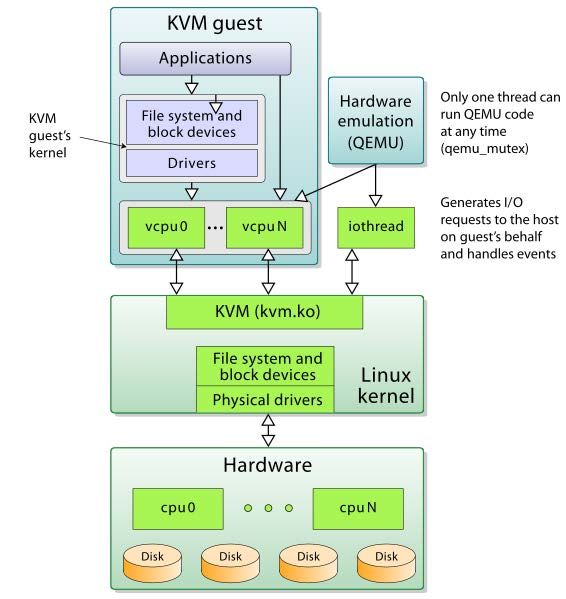
\includegraphics[width=0.8\textwidth]{imgs/3.1.jpg}}
    \caption*{\textit{\href{https://commons.wikimedia.org/wiki/File:Kernel-based_Virtual_Machine.svg}{A high-level overview of the KVM/QEMU virtualization environment}}}
    \label{3.1}
\end{figure}

\subsubsection*{Установка гипервизора}
\addcontentsline{toc}{subsubsection}{Установка гипервизора}

Как мы говорили выше, гипервизор на основе KVM состоит из двух основных частей: модуля ядра
Linux и QEMU, а потому подготовка хозяйской системы сводится к установке двух указанных
компонентов при помощи доступного в данном Linux-дистрибутиве пакетного менеджера.

Инструкции для широко распространённых дистрибутивов:
\begin{itemize}
    \item \href{https://help.ubuntu.ru/wiki/kvm}{Ubuntu};
    \item \href{https://wiki.debian.org/ru/KVM}{Debian};
    \item \href{https://docs.fedoraproject.org/en-US/quick-docs/getting-started-with-virtualization/}{Fedora};
    \item \href{https://access.redhat.com/documentation/en-us/red_hat_enterprise_linux/7/html/virtualization_deployment_and_administration_guide/index/}{Red Hat};
    \item \href{https://wiki.centos.org/HowTos/KVM}{CentOS};
    \item \href{https://doc.opensuse.org/documentation/leap/virtualization/single-html/book.virt/index.html#sec-vt-installation-kvm}{openSUSE};
\end{itemize}

Возможно, вы уже заметили существенное отличие от рассмотренных ранее гипервизоров: KVM
можно с лёгкостью установить на любом более-менее современном Linux-дистрибутиве. На
некоторых не очень современных дистрибутивах его тоже можно установить, например, даже в
CentOS 5. Это делает KVM более удобным вариантом, чем Xen, не говоря уже о привередливом к
аппаратуре VMware ESXi.

\subsubsection*{Использование гипервизора}
\addcontentsline{toc}{subsubsection}{Использование гипервизора}

Как это бывает с любым ПО с открытым исходным кодом, вокруг KVM и QEMU было разработано
\href{http://www.linux-kvm.org/page/Management_Tools}{множество разнообразного инструментария}. Есть решения на любой вкус: командная строка (libvirt),
графический клиент (virt-manager), веб-интерфейс (Proxmox VE) и т. д.

Для многих из имеющихся инструментов существует неплохая открытая документация, а потому
заострять внимание на каком-то из них не имеет особого смысла.

\begin{figure}[h]%current location
    \centering
    \scalebox{1}{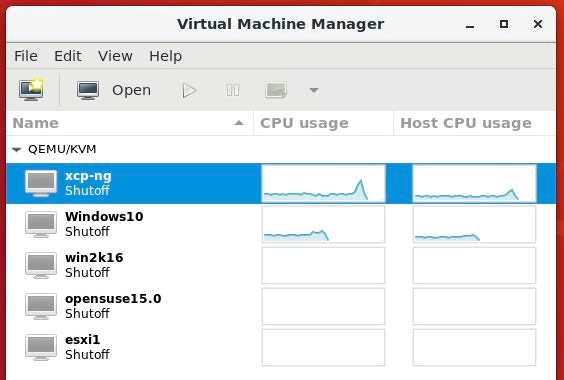
\includegraphics[width=0.8\textwidth]{imgs/3.2.jpg}}
    \label{3.1}
\end{figure}

\subsubsection*{Создание виртуальных машин}
\addcontentsline{toc}{subsubsection}{Создание виртуальных машин}

При помощи инструментария с графическим интерфейсом пользователя можно с лёгкостью создать
виртуальную машину, следуя предлагаемым шагам. Каждый инструмент имеет свои особенности, но в
целом не должно возникнуть сложностей. В отличие от ранее рассмотренных гипервизоров, в случае
KVM не существует стандарта де-факто, но вместо этого есть разнообразные варианты
использования, каждый из которых хорош по-своему: Proxmox VE, oVirt и т. д.

Сообществом разработчиков были созданы инструменты для импорта практически любых готовых
образов виртуальных машин и их дисков. «Всеядность» становится ещё одним преимуществом KVM,
в отличие от проприетарных гипервизоров, таких как VMware ESXi и Microsoft Hyper-V.

\subsubsection*{Создание виртуальных машин}
\addcontentsline{toc}{subsubsection}{Создание виртуальных машин}

Благодаря своей гибкости и использованию самых совершенных механизмов ядра Linux для
управлениями ресурсами аппаратуры, гипервизор на основе KVM завоёвывает всё большую часть
рынка серверной виртуализации. Как ранее отмечалось, компания Amazon перешла с использования
Xen на KVM, Google использует гипервизор KVM в основе своего сервиса Google Cloud, крупнейшие
хостинг-провайдеры, такие как Digital Ocean, используют KVM как основной гипервизор. Кроме того,
стоит помнить о том, что разработка KVM в значительной степени спонсируется компанией Red Hat,
ввиду того, что Red Hat предлагает своим клиентам решения для виртуализации на основе,
собственно, KVM. Более того, с недавних пор Red Hat стала частью IBM, а потому можно себе
представить, насколько серьёзные игроки заинтересованы в развитии и продвижении KVM.\newpage

\section*{Заключение о гипервизорах первого типа}
\addcontentsline{toc}{section}{Заключение о гипервизорах первого типа}

Как мы увидели из обзора нескольких гипервизоров первого типа, все они:
\begin{itemize}
    \item ориентированы на виртуализацию серверов, а не рабочих станций, что было характерной
    чертой гипервизоров второго типа;
    \item обладают развитыми средствами управления, в том числе, удалённого и централизованного;
    \item могут эффективно использоваться в вычислительных кластерах, обеспечивая эффективное
    масштабирование вычислительных ресурсов и повышенную надежность системы в целом.
\end{itemize}

\section*{Используемые источники}
\addcontentsline{toc}{section}{Используемые источники}

\begin{enumerate}
    \item \href{https://lwn.net/Articles/705160/}{Ten years of KVM}.
    \item \href{https://developer.ibm.com/articles/l-virtio/}{Virtio: An I/O virtualization framework for Linux}.
    \item \href{https://github.com/MicrosoftDocs/Virtualization-Documentation/raw/master/tlfs/Hypervisor%20Top%20Level%20Functional%20Specification%20v5.0C.pdf}{Hypervisor Top Level Functional Specification}.
    \item \href{https://github.com/MicrosoftDocs/Virtualization-Documentation}{Microsoft Virtualization documentation}.
\end{enumerate}

\section*{Используемые источники}
\addcontentsline{toc}{section}{Используемые источники}

\begin{enumerate}
    \item В чём преимущества и недостатки микроядерных гипервизоров по сравнению с монолитным
    вариантом?
    \item Какие возможности ядра Linux использует гипервизор KVM для своей работы?
    \item[3*.] Установите рассмотренные на занятии гипервизоры Microsoft Hyper-V, Xen, KVM и выполните
    измерения производительности гостевых систем в них.
\end{enumerate}

\end{document}